\chapter{Conclusion \fancyand~Open Problems}
\label{ch:conclu-automatic}

\begin{chapterpresentation}
	\begin{abstract}
		This part concludes \Cref{part:automatic} of this thesis.
		We recall some open problems mentioned in previous chapter,
		and highlight a new research direction relating the
		structural properties of a language-theoretic framework
		with its expressiveness.
	\end{abstract}
	% \medskip
	% \begin{acknowledgements}
	% \end{acknowledgements}
	\par\bigskip\bigskip
	\chaptertoc
\end{chapterpresentation}

\section{Separating Automatic Relations by Recognizable Ones}

\begin{marginfigure}
	\centering
	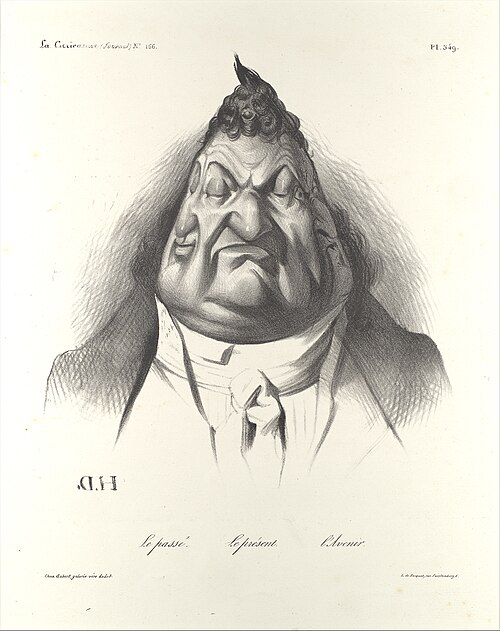
\includegraphics[width=\linewidth]{fig/PastPresentFuture.jpg}
	\caption{\href{https://www.metmuseum.org/art/collection/search/365043}{\emph{Le passé – Le présent – L'Avenir}}, Honoré Daumier, public domain.}
\end{marginfigure}
The problem introduced in \Cref{ch:preliminaries-automatic-structures}
remains open.

\openProblemAutRecSeparability*

In \Cref{ch:dichotomy-theorem}, we proved this problem to be equivalent
to "finite regular colourability of automatic graphs" (\Cref{thm:reg-colourability-equiv-separability}),
and showed that when the number of colours is fixed, the problem is undecidable
(\Cref{thm:k-reg-col-undec}).
In fact, we showed that most problems of this form are undecidable
(\Cref{thm:dichotomy-theorem-automatic-structures}).
However, as explained in \Cref{sec:dichotomy-discussion}, some gaps remain to be able to use
our techniques to prove the undecidability of the "$\AUT$/$\REC$-separability problem".

On the other hand, we introduced in \Cref{ch:algebra} an algebraic approach for
"automatic relations", hoping to prove the decidability of this problem.
Algebraic language theory is a powerful tool to prove the decidability of separation
over finite words \cite{PlaceZeitoun2016SeparatingRegularLanguages},
but also in more complex settings such as countable ordinal words \cite{ColcombetGoolMorvan2022FOSeparation}.

Alas, using the theory we developped to tackle \Cref{opb:AUT-REC-separability}
seems non-trivial. The main obstacle being that, while
"recognizable relations" have some desirable closure properties,
they do not form a "pseudovariety of automatic relations".
% \todo{addref-discuss-algebra}.%
% \footnote{Explain why we couldn't know this \emph{a priori}.}

Overall, Problem~\ref{opb:AUT-REC-separability} remains open.
Should this problem be decidable, the question of
the decidability of its generalization to larger class of relations would be
a natural next step.

\begin{openproblem}
	Are the "$\DRAT$/$\REC$-separability@@pb" and
	"$\RAT$/$\REC$-sepa\-ra\-bility problems" decidable?
\end{openproblem}

In \cite[\S~1]{BarceloFigueiraMorvan2023SeparatingAutomatic},
we incorrectly stated that ``As for definability\footnote{Definability is the same
as the "membership problem".}, the "$\REC$-separability problem" for "rational relations" is in general undecidable'', which is false---or at least we do not know it to be true.

Indeed, as mentioned in \Cref{ch:preliminaries-automatic-structures},
the "$\RAT$/$\REC$-membership problem" is undecidable, by
\cite[\S~III, Theorem~8.4]{Berstel1979Transductions}.
Moreover, in general, "membership problems" reduced to "separability problems":
a relation $\+R$ belongs to a class $\+V$ if, and only if, $\+R$ and $\negrel \+R$
are "$\+V$-separable@@rel". However, for this argument to work, the larger class of relation
needs to be effectively closed under complement.
This is not the case of "rational relations", see \Cref{sec:prelim-rational-relations}.

For "deterministic rational relations", while they are effectively
closed under complementation, the "$\DRAT$/$\REC$-membership problem"
is decidable---see \Cref{sec:prelim-automatic-dret}!

\section{Colouring Problems on Automatic Graphs}

Let us quickly recall some of the conjectures that have been discussed in \Cref{sec:dichotomy-discussion}.
The first one is about finding an equivalent characterization in the "dichotomy theorem
for automatic structures" (\Cref{thm:dichotomy-theorem-automatic-structures}).

\conjInvarianceGraphIsomorphisms*

In other words, this problem could be rephrased as follows: ``is a problem
of the form $\HomRegAut{\?B}$ decidable if, and only if, its output
only depends on the "structure represented" by the "automatic presentation",
and not on the "presentation@@auto" itself?''

Going back to out original question,
while we do not know if "finite regular colourability of automatic graphs"
is decidable, it is natural to study variations of this problem, as well as
sufficient or necessary conditions to ensure colourability or non-colourability.
Unfortunately, these problems are also non-trivial.

\conjFiniteColourabilityUndecidable*

\conjUnboundedCliques*

\section{An Algebraic Approach Beyond Automatic Relations}

The algebraic theory developed in \Cref{ch:algebra} can be generalized,
by replacing the constraint of ``being "well-formed"'' with an arbitrary
"regular language" $\Omega$. This would result in the notion
of \AP""$\Omega$-path algebras""---with "$\WellFormed$-path algebras" corresponding
to our "synchronous algebras".

While there is no hope to get a version of the
"lifting theorem" (\Cref{thm:lifting-theorem-monoids}) for every $\Omega$---see \Cref{rk:no-algo-lifting}, we believe it holds for "fully-preordered languages".
See \Cref{sec:algebra-discussion} for more details.

Interestingly, we believe this question to be related to Figueira \& Libkin's
"$T$-controlled relations", presented in
\Cref{sec:preliminaries-automatic-structures-relations-restricted-head-movements}.
We believe that each language $T$, specifying the head movements that are allowed,
gives rise to a language $\Omega_T$, such that relations recognized
by finite "$\Omega_T$-path algebras" exactly correspond to 
the "$T$-controlled relations".
\opbControlledRelations
We think that, one way of tackling this problem would be study properties of
the category of "$\Omega_T$-path algebras".

\conjAdjunctionControlledRelations*

Hopefully, the latter condition could maybe be massaged to get decidability.


\section{Theorem Projection via Monad Adjunction}

In fact, the conjecture of \Cref{conj:controlled-relations-category-equivalence}
is part of a larger idea we have, about relating the expressiveness of
universe---formalized by a monad---and its categorical properties. 
In algebraic language theory, monads play an essential role---see \Cref{apdx:monads}.
Informally, a monad describes a universe.
For instance, the monad
\[
	\Sigma \mapsto \Sigma^*
\]
describes the universe of finite words, and gives rise to the notion of
"monoids". Similarly, weighted words over a field $\symbb{K}$ can be described by
\[
	\Sigma \mapsto \symbb{K}\Sigma^*,
\]
where $\symbb{K}X$ denotes the free vector space over set $X$.
Again, this monad gives rise to Reutenauer's ``algèbres associatives''
\cite{Reutenauer1980SeriesFormelles}, "aka" ``$\symbb{K}$-weighted monoids'',
which is essentially an algebraic structure that is both a monoid and a
$\symbb{K}$-vector space.
Our "synchronous algebras" are no exception---see \Cref{apdx:monads}---,
and we refer the reader to \cite[\S~4]{Bojanczyk2020MSO} for more examples.

For well-behaved monads, ``languages'' recognized by their finite algebras
coincide with "monadic second-order"-definable languages.%
\footnote{We refer here to \emph{external} logics in the sense of
\Cref{rk:internal-vs-external-logic}.}
This gives rise to a natural set of questions, consisting
in finding algebraic characterizations
of fragments of "monadic second-order logic".
The perhaps most celebrated example is that of
the Schützenberger-McNaughton-Papert theorem
proves that "first-order"-definable languages of finite words
are exactly those recognized by aperiodic monoids
\cite{Schutzenberger1965FiniteMonoidsAperiodic,McNaughtonPapert1971CounterFreeAutomata}.
The statement was extended to $\omega$-words \cite{Perrin1984Recent},
to countable ordinal words \cite{Bedon2001Logic},
and to countable scatter words \cite{BesCarton2011AlgebraicFO}.
In the latter case, asking only for aperiodicity is not enough:
the algebra should also be ``gap-insensitive''.%
\footnote{In the more general case of words over countable orderings,
Colcombet and Sreejith also provides a characterization for "first-order"
definable languages, although it is more complex \cite{ColcombetSreejith2015Limited}.}
This can be explained as follows: by going from the simpler setting
of finite words (or countable ordinal words) to countable scattered words,
there are new phenomena that appear and that "first-order logic" is 
not able to describe.

However, intuitively, going in the other direction should be easy!
Given an algebraic characterization of first-order logic over a ``richer'' monad
("eg" countable scatter words), it should be easy to reprove the
Schützenberger-McNaughton-Papert theorem over finite words, using the
``rich'' algebraic characterization as a black box.

\begin{marginfigure}
	\centering
	\begin{tikzpicture}
		\node at (0,0) (base) {\small``base monad''};
\node[right=3em of base] (rich) {\small``richer monad''};

\draw[edge] (base) to[bend left=30] node[midway, above] {\small encoding} (rich);
\draw[edge] (rich) to[bend left=30] node[midway, below] {\small projection} (base);
	\end{tikzpicture}
	\caption{
		\AP\label{fig:adjunction-informal}
		Tools to project algebraic characterizations from one universe to another.
	}
\end{marginfigure}
Surprisingly, while it is easy to ``project'' the algebraic characterization
of first-order logic over $\omega$-words to get its counterpart for finite words,
the task becomes less straightforward---but still possible---when projecting from
countable ordinal words or countable scattered words to finite ones.
In both cases, the proof relies on two ingredients:
\begin{itemize}
	\item a function, encoding a language of finite words into
		a language in the richer setting;
	\item a function, projecting a language in the richer setting
		to a language of finite words,
\end{itemize}
see \Cref{fig:adjunction-informal}.
Moreover, both functions should preserve the properties that we are studying---either
being "first-order" definable, or satisfying the algebraic characterization.

In the case of $\omega$-words, finding these functions is easy: for instance, 
the projection simply consists in restricting a language of words of
length at most $\omega$ to the finite words.
On the other hand, the projection from countable scattered words
to finite ones cannot simply do this, since finite words are not
"first-order" definable amongst countable scattered ones.
Hence, the projection in question needs to be tailor-made to 
preserve first-order logic.\footnote{This construction is an unpublished joint
work with Thomas Colcombet.}

In fact, the projection of $\omega$-words to finite words does not only preserve
the property of being "first-order" definable, but more generally any
"pseudovariety@@reglang"! In this sense, words of length at most $\omega$
form a \emph{conservative extension} of finite words, while
countable scattered words do not: this is why we can find a single construction
to project algebraic characterizations%
\footnote{By ``algebraic characterization'' we formally mean an "Eilenberg-Schützenberger correspondence@@lang".}
from $\omega$-words to finite ones, but not from countable scattered words to finite ones.

This begs the question: how can we formalize this idea of a monad being
a \emph{conservative extension} of another one?
In light of \Cref{fig:adjunction-informal} propose to look at the notion of "monad adjunction".
Before introducing it, we need a preliminary definition.

Let $\Monad[S] = (S,\unit,\mult)$ be a $\cat{C}$-monad
and $\Monad[T] = (T,\unit,\mult)$ be a $\cat{D}$-monad.%
\footnote{Following Street, we use the same notation for the unit and multiplication in $\Monad[S]$ and $\Monad[T]$.}
We assume $\cat C$ and $\cat D$ to be both categories of typed sets.

A \AP""monad functor"",%
\footnote{The notion was introduced by Street \cite[\S 1]{Street1972Monads}
in the slightly more general context of 2-categories.
We found this reference thanks to \cite{Rezk2012Functors}. "Monad functors" are also known as
``lax maps of monads''.}
from $\Monad[S]$ to $\Monad[T]$ is a pair $(\Phi, F)$, where:
\begin{itemize}
\item $F\colon \cat{C} \to \cat{D}$ is a functor,
\item $\Phi\colon TF \Rightarrow FS$ is a natural transformation,
\end{itemize}
such that, for every object $X \in \cat{C}$, the following diagrams commute:\\
\begin{center}
	\intro*\textup{\MFunit:}
	\begin{tikzcd}
		FX \ar[d,"{\unit[FX]}" swap] \ar[dr, "{F\unit[X]}"] & \\
		TFX \ar[r,"\phi_{X}" swap] & FSX,\\
	\end{tikzcd}
	\quad\intro*\textup{\MFmult:}
	\begin{tikzcd}[row sep=large, column sep=-.2em]
		& & TFSX \ar[rr, "\phi_{SX}"] & &  FSSX \ar[drr, "{F\mult[X]}", bend left=0] \\
		TTFX \ar[urr, "T\phi_X", bend left=0] \ar[drrr, "{\mult[FX]}" swap, bend right=0] & &
			& & & & FSX. \\[-.5em]
		& & & TFX \ar[urrr, "\phi_X" swap, bend right=0]
	\end{tikzcd}
\end{center}

Such a pair is denoted by $\intro*\MF{\Phi}{F}\colon \Monad[S] \Rightarrow \Monad[T]$.%
\footnote{Note that, somewhat surprisingly, one element of a monad functor
from $\Monad[S]$ to $\Monad[T]$ goes is covariant---namely the functor
$F\colon \cat{C} \to \cat{D}$---while the other one is contravariant---namely
the natural transformation $\Phi\colon TF \Rightarrow FS$. The next example will
illustrate why this definition makes sense.}
% \begin{marginfigure}
% 	\centering
% 	\intro*\textup{\MFunit:}
% 	\begin{tikzcd}
% 		FX \ar[d,"\unit_{FX}" swap] \ar[dr, "F\unit_{X}"] & \\
% 		TFX \ar[r,"\phi_{X}" swap] & FSX.\\
% 	\end{tikzcd}\\
% 	\intro*\textup{\MFmult:}
% 	\begin{tikzcd}[row sep=large, column sep=0em]
% 		& & TFSX \ar[rr, "\phi_{SX}"] & &  FSSX \ar[drr, "F\mult_X", bend left=0] \\
% 		TTFX \ar[urr, "T\phi_X", bend left=0] \ar[drrr, "\mult_{FX}" swap, bend right=0] & &
% 			& & & & FSX. \\
% 		& & & TFX \ar[urrr, "\phi_X" swap, bend right=0]
% 	\end{tikzcd}
% 	\caption{
% 		\AP\label{fig:axioms-monad-functor}
% 		Axioms of a "monad functor".}
% \end{marginfigure}

\begin{marginfigure}
	\centering
	\begin{tikzpicture}
		\node at (0,0) (base) {$\MonadPlus$};
\node[right=3em of base] (rich) {$\MonadWilke$};

\draw[edge] (base) to[bend left=30] node[midway, above] {$\MFzero$} (rich);
\draw[edge] (rich) to[bend left=30] node[midway, below] {$\MFproj$} (base);
	\end{tikzpicture}
	\caption{
		\AP\label{fig:adjunction-informal-finite-wilke}
		"Monads functors" between "Kleene's monad" and "Wilke's monad".
	}
\end{marginfigure}
\begin{example}[Finite words and $\omega$-words]
	Let $\intro*\MonadPlus$ be ""Kleene's monad"" over the category $\Set[]$
	of non-empty finite words,
	defined by $X \mapsto X^+$. Moreover, let $\intro*\MonadWilke$ be ""Wilke's monad"",
	defined over the category of "2-typed sets" $\Set[+,\omega]$, by
	$\tup{F,I} \mapsto \tup{F^+, F^+I \cup F^{\omegafin}}$, where \AP$F^{\intro*\omegafin}$
	denotes the set of ultimately-periodic words of length $\omega$ over $F$.

	We start by defining a "monad functor" from $\MonadWilke$
	to $\MonadPlus$: it represents the natural surjection
	from words of length at most $\omega$ to non-empty finite words.
	Let $\intro*\projMon\colon \Set[+,\omega] \to \Set$ be the functor that only keeps the first component, defined by $\tup{F,I} \mapsto F$, and $\Phi$ be the natural transformation
	$\MonadPlus\projMon \Rightarrow \projMon\MonadWilke$, defined for $\tup{F,I} \in \Set[+,\omega]$
	by letting
	\[
		\begin{tikzcd}[column sep=small]
			\phi_{F,I}\colon
			\underbrace{\MonadPlus\projMon \tup{F,I}}_{= F^+} \rar &
			\underbrace{\projMon\MonadWilke \tup{F,I}}_{= F^+}
		\end{tikzcd}
	\]
	be the identity. Then $\intro*\MFproj$ is a "monad functor" from
	"Wilke's monad" to "Kleene's monad".

	Dually, we then define a "monad functor" from $\MonadPlus$
	to $\MonadWilke$ that corresponds to the
	natural embedding of non-empty finite words into words of length at most $\omega$.
	We let \AP$\intro*\zero\colon \Set[] \to \Set[+,\omega]$ be the functor that transforms a
	set $X$ into a pair $\tup{X,\set{\bullet}}$, and $\Psi$ be the natural transformation
	$\MonadWilke\zero \Rightarrow \zero\MonadPlus$, defined for $X \in \Set[]$ by letting
	\[
		\begin{tikzcd}[column sep=small]
			\psi_{X}\colon
			\underbrace{\MonadWilke\zero X\vphantom{\MonadPlus}}%
				_{=\tup{X^+, X^+\set{\bullet} \cup X^{\omegafin}}} \rar &
			\underbrace{\zero\MonadPlus X}%
				_{=\tup{X^+, \set{\bullet}}}
		\end{tikzcd}
	\]
	send $u \in X^+$ to itself, and $u \in X^+\set{\bullet} \,\cup\, X^{\omegafin}$ to $\bullet \in \set{\bullet}$. Then $\intro*\MFzero$ is a "monad functor" from
	"Kleene's monad" to "Wilke's monad", see \Cref{fig:adjunction-informal-finite-wilke}.
\end{example}

Unsurprisingly, "monad functors" can be composed. Moreover, 
it can be shown that any "monad functor" from $\Monad[S]$ to $\Monad[T]$ induces
a functor from the category of $\Monad[S]$-algebras to $\Monad[T]$-algebras.
For instance, $\MFproj\colon \MonadWilke \Rightarrow \MonadPlus$ induces
the functor from Wilke's algebras to semigroups that sends $\tup{S^+,S^\omega}$
to $S^+$.
Dually, $\MFzero\colon \MonadPlus \Rightarrow \MonadWilke$ induces the functor
from semigroups to Wilke's algebras that sends $S$ to $\tup{S, \set{\bullet}}$.

I conjecture that we can naturally define a notion of ``monad (functor) adjunction'',
which generalizes the notion of ``functor adjunctions'',
in such a way that a \AP""monad adjunction"" between $\Monad[S]$ and $\Monad[T]$
induces an adjunction between $\Monad[S]$-algebras and $\Monad[T]$-algebras.
A typical example of such a "monad adjunction" would be
\Cref{fig:adjunction-informal-finite-wilke}.

\begin{marginfigure}
	\centering
	\begin{tikzpicture}
		\node[font=\footnotesize] at (0,0) (base) {semigroups};
\node[right=3em of base, font=\footnotesize] (rich) {Wilke's algebras};

\draw[edge] (base) to[bend left=30] node[midway, above, font=\footnotesize] {$R \mapsto \tup{R,\set{\bullet}}$} (rich);
\draw[edge] (rich) to[bend left=30] node[midway, below, font=\footnotesize] {$\tup{L^+, L^\omega} \mapsto L^+$} (base);
	\end{tikzpicture}
	\caption{
		\AP\label{fig:adjunction-formal-finite-wilke}
		An adjunction between the category of
		$\MonadWilke$-algebras and the category of $\MonadPlus$-algebras.
	}
\end{marginfigure}
``Monad (functor) adjunctions'' are high-order objects, and so for the sake
of simplicity, we will work with the adjunction they induce between the categories
algebras. We go back to the example of \Cref{fig:adjunction-informal-finite-wilke}:
we represent in \Cref{fig:adjunction-formal-finite-wilke} the two functors induced
between their Eilenberg-Moore categories.
It is indeed an adjunction, with $\tup{L^+, L^\omega} \mapsto L^+$ acting as the left
adjoint and $R \mapsto \tup{R,\set{\bullet}}$ as the right adjoint, and there
are \emph{natural} bijections
\[
	\textrm{hom}_{\cat{Sgp}}(L^+, R)
	\cong \textrm{hom}_{\cat{Wilke}}(\tup{L^+,L^\omega}, \tup{R,\bullet}).
\]

We believe that this adjunction are precisely what allows us to automatically project
any algebraic characterization of $\omega$-regular languages to an algebraic
characterization of "regular languages"---for a good reason: 
the two maps $\tup{L^+, L^\omega} \mapsto L^+$ and $R \mapsto \tup{R,\set{\bullet}}$
are the key ingredient of the proof!

Interestingly, sending a semigroup $S$ to the ordinal semigroup
$S \dcup \{\textbullet\}$, defined by letting any infinite product
be equal to the zero element $\textbullet$ also defines a functor
from the category of semigroups to the category of ordinal semigroups.
Dually, the canonical surjection sending an ordinal semigroup to
its underlying semigroup is a functor from
the category of ordinal semigroups to the category of semigroups.
However, they do not form an adjunction!
We actually believe that there are no adjunction between these categories.

\begin{marginfigure}
	\centering
	\includegraphics[width=\linewidth]{fig/Sieste.jpg}
	\caption{\href{https://commons.wikimedia.org/wiki/File:Henri_Manguin,_1905,_La_Sieste_(Le_repos,_Jeanne),_oil_on_canvas,_88.9_x_116.84_cm,_Villa_Flora,_Winterthur.jpg}{\emph{La Sieste}}, Henri Manguin, public domain.}
\end{marginfigure}
These observations lead us to the last conjecture of this thesis.
\begin{conjecture}[Projecting algebraic characterizations]
	\AP\label{conj:projecting-algebraic-characterizations}
	Let $\Monad[S]$ and $\Monad[T]$ be two monads.
	Any monad adjunction between them induces
	a ``natural function'' from "Eilenberg-Schützenberger correspondences@@lang" over $\Monad[T]$
	to "Eilenberg-Schützenberger correspondences@@lang" over $\Monad[S]$.
\end{conjecture}

In the case of finite words and $\omega$-words, this
surjection sends for instance the theorem
``an $\omega$-regular language is first-order definable "iff" its
syntactic Wilke's algebra is aperiodic'' onto the theorem
``a "regular language" is first-order definable "iff" its
syntactic semigroup is aperiodic''!
We believe that the "lifting theorem" (\Cref{thm:lifting-theorem-monoids-pseudovarieties})
of the previous chapter could be a consequence of
\Cref{conj:projecting-algebraic-characterizations}.